\documentclass[titlepage,12pt,ceqn]{article}%

\usepackage[english]{babel}
\usepackage{setspace}
\usepackage{graphicx}
\usepackage{epsfig}
\usepackage{amssymb}
\usepackage{amsmath}
\usepackage{graphics}
\usepackage{units}
\usepackage{commath}
\usepackage{multirow}
\usepackage{booktabs}
\usepackage{caption3} % load caption package kernel first
\usepackage[small]{caption}
\usepackage{array}
\everymath{\displaystyle}
\usepackage[final]{pdfpages}


%\pagestyle{headings}
\setlength{\oddsidemargin}{0in}
\setlength{\evensidemargin}{-0.25in}
\setlength{\topmargin}{-0.25in}
\setlength{\textheight}{8.85in}
\setlength{\textwidth}{6.75in}
\setlength{\footskip}{0.75in}
%\newfont{\footfont}{cmmi10 at 40pt}
%\makeatletter
%\def\writewhite{\special{ps: gsave 1 setgray}}
%\def\writeblack{\special{ps: 0 setgray grestore}}
%\def\writegray{\special{ps: gsave 0.7 setgray}}
%\renewcommand{\@oddfoot}{\hfill\mbox{\vbox to 1cm{\writegray
%                         \hrule height 1cm width 1cm}
%                         \hspace*{-1cm}\writewhite\raisebox{5pt}{\footfont{\symbol{25}}}}
%                         \hfill\writeblack}
%\renewcommand{\@evenfoot}{\hfill\mbox{\vbox to 1cm{\writegray
%                         \hrule height 1cm width 1cm}
%                         \hspace*{-1cm}\writewhite\raisebox{5pt}{\footfont{\symbol{25}}}}
%                         \hfill\writeblack}
%\makeatother
\DeclareCaptionOption{parskip}[]{} % disable "parskip" caption option

%differentiation
\makeatletter
\providecommand*{\diff}%
    {\@ifnextchar^{\DIfF}{\DIfF^{}}}
\def\DIfF^#1{%
    \mathop{\mathrm{\mathstrut d}}%
        \nolimits^{#1}\gobblespace}
\def\gobblespace{%
    \futurelet\diffarg\opspace}
\def\opspace{%
    \let\DiffSpace\!%
    \ifx\diffarg(%
        \let\DiffSpace\relax
    \else
        \ifx\diffarg[%
            \let\DiffSpace\relax
    \else
        \ifx\diffarg\{%
            \let\DiffSpace\relax
        \fi\fi\fi\DiffSpace}

\providecommand*{\deriv}[3][]{%
    \frac{\diff^{#1}#2}{\diff #3^{#1}}}

\providecommand*{\pderiv}[3][]{%
\frac{\partial^{#1}#2}%
{\partial #3^{#1}}} 


\begin{document}

\begin{titlepage}
	\begin{center}
	\line(1,0){470}\\
	\Huge{\bfseries	 Statistics Without Agonizing Pain}\\
	[6cm]
    \textsc{ UNIVERSITY OF TORONTO}\\
    [1cm]
	\textmd{\large SCS 3030: Big Data Tools and Techniques\\
	 Mining Financial, Operational and Social Network Data}\\
	[6cm]
	\textsc{\large{Jamil Antoine Jabbour\\
			December 10, 2016 }}
	\end{center}
\end{titlepage}

\doublespace
\section{Introduction}
This report investigates the thesis that if a computer can be programmed, then we have direct access to the deepest and fundamental ideas in statistics. To examine this thesis, a problem with a statistical argument is needed. The argument to be resolved is whether drinking beer makes humans more attractive to malarial mosquitoes. This study is of interest due to the rising of alcohol consumption in developing countries and malaria still being the leading cause of mortality~\cite{feachem2008new} and~\cite{world2008}. After all, malaria is transmitted via mosquitoes. In this report, a statistical analysis and a numerical approach are presented to investigate the hypothesis in the study by Lef\`evre \textit{et al.}~\cite{lefevre2010beer}.

Historically, most studies for malarial transmission have assumed that all individuals are at an equal risk for mosquito bites \cite{MalriaHistory} and \cite{Mathbifurcation}. However, current studies have provided evidence that human beings vary widely in their ability to attract mosquitoes. Thus understanding which individuals are at a greater risk for mosquito bites becomes crucial in targeting interventions more accurately in the fight against malaria. Identifying these causes could possibly control and reduce the mortality rate.

The study by Lef\`evre \textit{et al.}~\cite{lefevre2010beer} has been conducted in Burkina Faso (West Africa) that investigated the effect of beer consumption on human attractiveness to malarial mosquitoes. The experiment involved 43 local male volunteers. The volunteers were divided into two subgroups; a group of 25 participants that consumed beer and a group of 18 participants that consumed water. The odour of the participants was blown through a fan into one fork of the Y-shaped tube, known as Y-olfactometer and air is blown in the other end of the fork. \textit{Anopheles} vectors, primary African malarial mosquitoes, are released at the opposite end of the Y-olfactometer. The vectors flying towards the two forks are trapped and the number of trapped mosquitoes in the fork exposed to the odour of participant are collected. A statistical analysis is conducted to check if the mean difference between the two groups is significant for the claim that beer consumption has an effect on human attractiveness to malarial mosquitoes. Section~\ref{stats} provides a brief overview of the experiment and the statistical analysis conducted.

%This experiment involved 43 male subjects divided into two subgroups where they were asked to consume alcohol or water to understand the link between malaria and alcohol consumption.
%This experiment is of interest due the rise in alcohol consumption in developing countries and malaria still being the leading cause of mortality. Different experiments showed strong evidence that humans vary in their attractiveness to malarial mosquitoes and understanding these causes could possibly control and reduce the mortality rate.
In this report, a different numerical approach is used to revoke or accept the results that the increase in human attractiveness to malarial mosquitoes is due to beer consumption. The hypothesis of the previous study will be investigated as an argument between two different views. One view of Lef\`evre \textit{et al.}~\cite{lefevre2010beer} claims that the mean difference is significant and beer consumption increases human attractiveness to malarial mosquitoes. The opposite view  claims that this difference is insignificant and it could have happened  due to chance. Section~\ref{computational} presents a detailed overview of the numerical approach that is implemented using the logic of the second claim. Finally, the results are summarized in Section~\ref{results}.

%The experiment and data used in this report are those presented in a study~\cite{lefevre2010beer}. The study "Beer Consumption Increases Human Attractiveness to Malaria Mosquitoes" presents an experiment that has been conducted in Burkina Faso (West Africa) to understand the links between malaria and alcohol consumption. In the effort to control malaria, many studies have been conducted and have shown that there is strong evidence that humans vary in their attractiveness to \textit{Anopheles} vectors
%In developing countries, alcohol consumption is rising and in an effort to manage malaria, studies  have been conducted to understand the links between malaria and alcohol consumption.

\section{Experiment}\label{Experiment}
A brief overview of the methodology and procedures of the experiment conducted by Lef\`evre \textit{et al.} are shown in subsection~\ref{method} and the statistical analysis is summarised in subsection~\ref{stats}.

\subsection{Methodology}\label{method}
The experiment was conducted in a semi-field condition in Burkina Faso and involved 43 local male volunteers. This experiment was designed to identify the effect of alcohol consumption on human attractiveness to malarial mosquito. An illustration of the apparatus of the experiment is shown in Figure~\ref{aparatus}.
\begin{figure}[ht]
\centerline{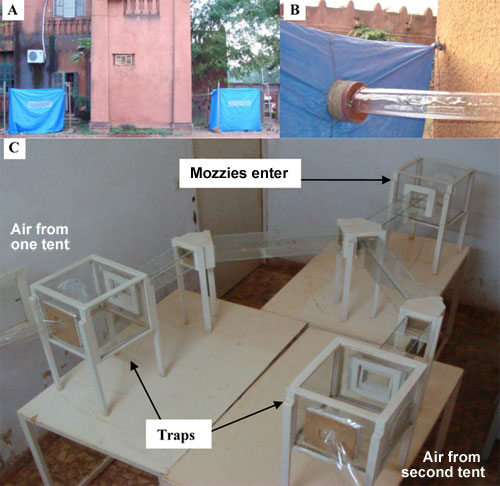
\includegraphics[height=8cm,width=12cm]{./Figures/aparatus}}
\caption{(A) Two tents are set up outdoors and connected to the two traps of the Y-olfactometer by lay-flat tubing. (B) Fan drawing air from a tent to the olfactometer. (C) The Y tube-olfactometer \label{aparatus}}
\end{figure}

The volunteers were divided into two subgroups, a group of 25 participants that consumed one litre of beer and another group of 18 participants that consumed one litre of water. The Y-olfactomer was located in an experimental room and connected to the outside by lay-flat tube.  The participants were seated in a tent shirtless for 30 minutes and their odour (sweat, breath, urine ...) were  blown into one fork of the Y-olfactometer. The other end of the fork is exposed to air. A batch of 50 \textit{Anopheles} vectors are released in the downwind box of the Y-olfactometer and given the choice between outdoor air and human odour. During the experiment time frame, mosquitoes that responded to the stimuli left the downwind box and flew upwind into the traps at the end of the Y-tube. The number of trapped vectors were collected and classified depending on the participants drink. The mean of both data is calculated and the mean difference is found. Subsequently, a statistical analysis was conducted to check if the calculated mean difference between the two groups is significant to claim that beer consumption has an effect on human attractiveness to mosquitoes.
%involved 43 male  It consists of the use of a Y tube-olfactometer to take advantage of the participants whole body scent (breath, skin …) as a stimulus to measure human attractiveness to Anopheles gambiae (the primary African malaria vector). The participants were divided into two subgroups, a group consists of 25 volunteers that consume beer and a total of 2500 mosquitoes and another group consists of 18 volunteers that drink water  and a total of 18000 mosquitoes. All volunteer were Burkinabe adult healthy males aged between 20 and 43 and the mosquitoes were female gambiae (3 to 4 days old) and are trapped in cages in group of 50. Figure~\ref{aparatus} shows an illustration of the experiment apparatus.


\subsection{Analytical Approach}\label{stats}
The mean difference of the two groups in the experiment is found to be approximately 4.4, which can be interpreted that the average person who drinks beer attracts 4.4 more mosquitoes than the average person who drinks water. Therefore, this investigation raises the statistical question of whether a difference of 4.4 is sufficient evidence to claim that drinking beer makes humans more attractive to mosquitoes. In addition, a different argument could be  established that the difference of 4.4 could have happened by chance leading to the conclusion that the beer consumption has no effect. In Section~\ref{stats}, this argument will be resolved using the analytical agonizing statistical approach that is conducted in this paper~\cite{lefevre2010beer} and in Section~\ref{computational}, using a simple numerical method.

Generally, Welch's test is conducted to investigate the hypothesis that the two populations with unequal variance and sample sizes have equal means. It is typically applied when the statistical units underlying the two samples being compared are non-overlapping. Thus, this test is applied to examine the hypothesis presented in the study \cite{lefevre2010beer}. This test starts by defining the null hypothesis $\mathit{{H_{0}}}$ and the alternative hypothesis $\mathit{{H_{1}}}$ as follows,
\begin{align*}
 &\mathbf{Null~Hypothesis:}  &  &\mathbf{Alternative~Hypothesis:}  \\
 &H_0: \bar{X_1} = \bar{X_2}, &  &H_1: \bar{X_1} \neq \bar{X_2},
\end{align*}
leading to computing two necessary values, the $t$-statistic value and the number of degree of freedom $\nu$. We compute the $t$-statistic value according to the formula,
\begin{equation*}
t = \frac{\bar{X_1}-\bar{X_2}}{\sqrt{\frac{{s^2_1}}{n_1} +\frac{{s^2_2}}{n_2}}},
\end{equation*}
where $s{_i^2}$ and $ n_{i}$ represent the sample variance and the sample size respectively. Then, we need to estimate the number of degree of freedom according to,
\begin{equation*}
\nu \approx \large \frac{\left(\frac{{s^2_1}}{n_1} +\frac{{s^2_2}}{n_2}\right)^2}{\left(\frac{s^2_1}{n_1}\right)^2\left(n_1 -1\right) + \left(\frac{{s^2_2}}{n_2}\right)^2\left(n_2 -1\right)}.
\end{equation*}
The degree of freedom value is needed to look up the critical value $t_c$ from the corresponding t-test table, and then compare it to the $t$-statistic value computed previously. If $t > t_{c}$ then it can be concluded that a difference of 4.4 additional mosquitoes is statistically significant with a confidence interval of $95\%$. The nominal parameters of the test are summarized in Table~\ref{Wttest}. Based on the Welch test, the study concluded that there is evidence with a confidence interval of 95\% that the beer consumption increases the human attractiveness to malarial mosquitoes.
\begin{table}[b]
\begin{center}
\caption{The nominal parameters used in Welch's test.\label{Wttest}}
\begin{tabular}{l|p{9.5cm}|l} \hline\hline\multicolumn{3}{c}{Welch's test parameters}\\
\hline Symbol & Parameter & Value \\ \hline
$\bar{X_b} - \bar{X_w}$ & The mean difference between beer and water samples & 4.4 \\
$t$ & $t$-statistic & 3.67\\
$t_c$ & The critical value of $t$ at 95\% confidence interval &  2.021\\
$\nu$ & Degree of Freedom &  39.1 \\ \hline
 \end{tabular} \end{center} \end{table}

\section{Numerical Approach}\label{computational}
In this section, a numerical approach is introduced which is different than the analytical approach described in Section~\ref{stats}. The statistical analysis conducted previously is based on some assumptions where $t$ is assumed to follow the following,
\begin{equation*}
  t(x,\nu) = \frac{\Gamma(\frac{\nu+1}{2})}{\sqrt{\nu\pi}\Gamma(\frac{\nu}{2})}\left(1 +\frac{x^2}{\nu} \right)^{-\frac{\nu+1}{2}},
\end{equation*}
where $\Gamma(x,t)$ is a probability function. The difficulties of understanding the random sampling distribution and the possibility of doubting the choice of the correct distribution under some assumptions motivate the numerical approach for this report. This approach is built on the argument that a 4.4 difference of additional mosquitoes in the mean difference could have happened due to chance and not from beer consumption. A detailed overview of the numerical approach is provided which was implemented using Python to support or reject the claim of the statistical analysis that beer consumption increases the human attractiveness to malarial mosquitoes.

In the case of a mean difference of 4.4 occurring due to chance, the data could be considered as labels and have no explicit information. Using this argument, the sampling distribution can be constructed by grouping the data, randomly shuffling them, splitting them into two groups, and computing the mean difference. Repeating this process many times allows for the unfolding  the sampling distribution. Figure~\ref{unfold} shows the process of unfolding the sampling distribution under the argument of mean difference of 4.4 occured due to chance.
\begin{figure}
  \centering
  \begin{tabular}{cc}
    \includegraphics[width=8cm]{./Figures/test0} & \includegraphics[width=8cm]{./Figures/test1} \\
     & \\
    \includegraphics[width=8cm]{./Figures/test2} & \includegraphics[width=8cm]{./Figures/test3} \\
  \end{tabular}
  \caption{shows the unfolding of the sampling distribution under the argument that the mean difference occurs to chance. The calculated mean difference of the shuffled data is plotted at every iteration.}\label{unfold}
\end{figure}

\subsection{Implementation}
The program is written using Python notebook and using its following libraries; pandas, numpy, random, and matplotlib. The data is divided into two attributes (beer and water) and is saved an excel format file. The document contains 25 entries corresponding to the subjects that drank beer and 18  entries corresponding to the 18 subjects that drank water.

The data is read to Python into two numpy arrays stored in a "Data Frame" using pandas library. Due to the difference in the number of entries of each attribute (25 and 18), these arrays are reshaped and stored into two different numpy array of corresponding size 25 and 18 to their attributes respectively.
The numerical approach consists of three main routines:
\begin{enumerate}
  \item Group the entries in one array of length 43 and randomly shuffle the entries.
  \item Split the data into two arrays of length 25 and 18 respectively.
  \item Compute the mean difference.
\end{enumerate}
This process is iterated $n$ times and the computed mean difference is plotted at every run. Doing so, we can see the sampling distribution unfolding under the argument that the mean difference occurred due to chance. Finally the proportion of obtaining a mean difference greater than 4.4 is calculated.

\begin{figure}[t]
\centerline{\includegraphics[height=8cm,width=16cm]{./Figures/Distribution_50k}}
\caption{shows the sampling distribution of the data under the argument that the mean difference of 4.4 between the two samples could have happened due to chance. \label{histogram}}
\end{figure}

\subsection{Results}\label{results}

In this section, the results of the numerical simulation are presented. The numerical solver first starts by importing the data and storing it as two numpy array of size 25 and 18 corresponding to the sample size of two groups of participants in the experiment described in Section~\ref{Experiment}. Then, three main routines are iterated for $n$ times. In the first routine, the two arrays are combined in one array of size 43 (25 +18), shuffled using a random permutation of the entries. The array with the permuted entries is split into two arrays with the original sample size 25 and 18. Finally, the mean difference of the two arrays containing the permuted data is calculated and stored at every iteration.
The calculated mean difference at every iteration and the mean difference of the experiment $\approx{4.4}$ are plotted. Figure~\ref{histogram} shows a sampling distribution when the numerical process is iterated 50000 times.

The numerical solver is executed many runs for different iteration values $n$. For every run, the calculated mean differences are compared to the mean difference of the experiment, 4.4. Therefore, the proportion $\alpha$ of having a mean difference greater than 4.4 can be calculated for every run. For the different runs, the proportion $\alpha$ is shown to be less 0.01 which leads us to reject the hypothesis that 4.4 mean difference occurred due to chance, thus supporting the conclusion of the result obtained in Lef\`evre \textit{at al.}~\cite{lefevre2010beer}; beer consumption increases human attractiveness to malarial mosquitoes. Figure~\ref{prop_0} and Table~\ref{result} shows the proportion of obtaining a mean difference greater than 4.4 at every simulation run.
\begin{table}[h]
\begin{center}
\caption{The nominal parameters of the numerical simulation.\label{result}}
\begin{tabular}{p{2cm}|p{7.5cm}|l}
\hline\hline Iteration number  & Calculated mean difference greater than the mean difference of the experiment   & Proportion \\
\hline $n$ & $X_w-X_b > 4.4 $ & $\alpha$ \\ \hline
500     & 1 & 0.002 \\
1000    & 0 & 0     \\
2500    & 0 & 0     \\
5000    & 3 & 0.0006\\
7500    & 1 & 0.0001333 \\
10000   & 5 &  0.0005   \\
25000   & 14&  0.00056 \\
50000   & 18&  0.00036 \\ \hline
 \end{tabular} \end{center} \end{table}

\begin{figure}[t]
\centerline{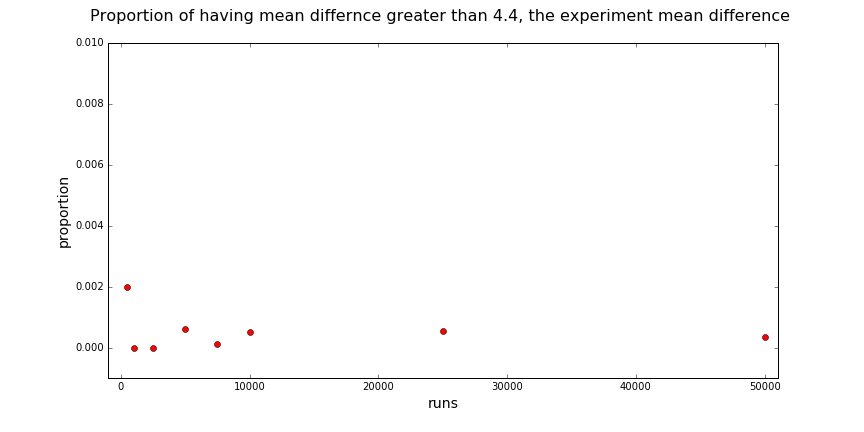
\includegraphics[height=8cm,width=16cm]{./Figures/proportion}}
\caption{shows the sampling distribution of the data under the argument that the mean difference of 4.4 between the two samples could have happened due to chance. \label{prop_0}}
\end{figure}

\subsection{Summary}
A numerical approach is implemented from scratch in Python notebook to investigate the results obtained by Lef\`evre \textit{et al.} using a statistical analysis approach. In order to implement the numerical solver and perform the statistic, it is required to follow three main tools and techniques.
\begin{enumerate}
  \item Ability to follow a simple logical argument.
  \item Ability to generate random number.
  \item Ability to repeat the process i.e. iteration.
\end{enumerate}
The first tool is acquired due to humans nature because humans uses logic as a unified language. The two following tools exist in any programming language with a decent library. Using these three simple tools and techniques, it is possible to understand the problem at a high level without using the analytical approach that requires years of studies to understand it. Therefore, being able to program a computer give us insights on understanding the fundamental ideas of statistics.

%input{main}
\newpage
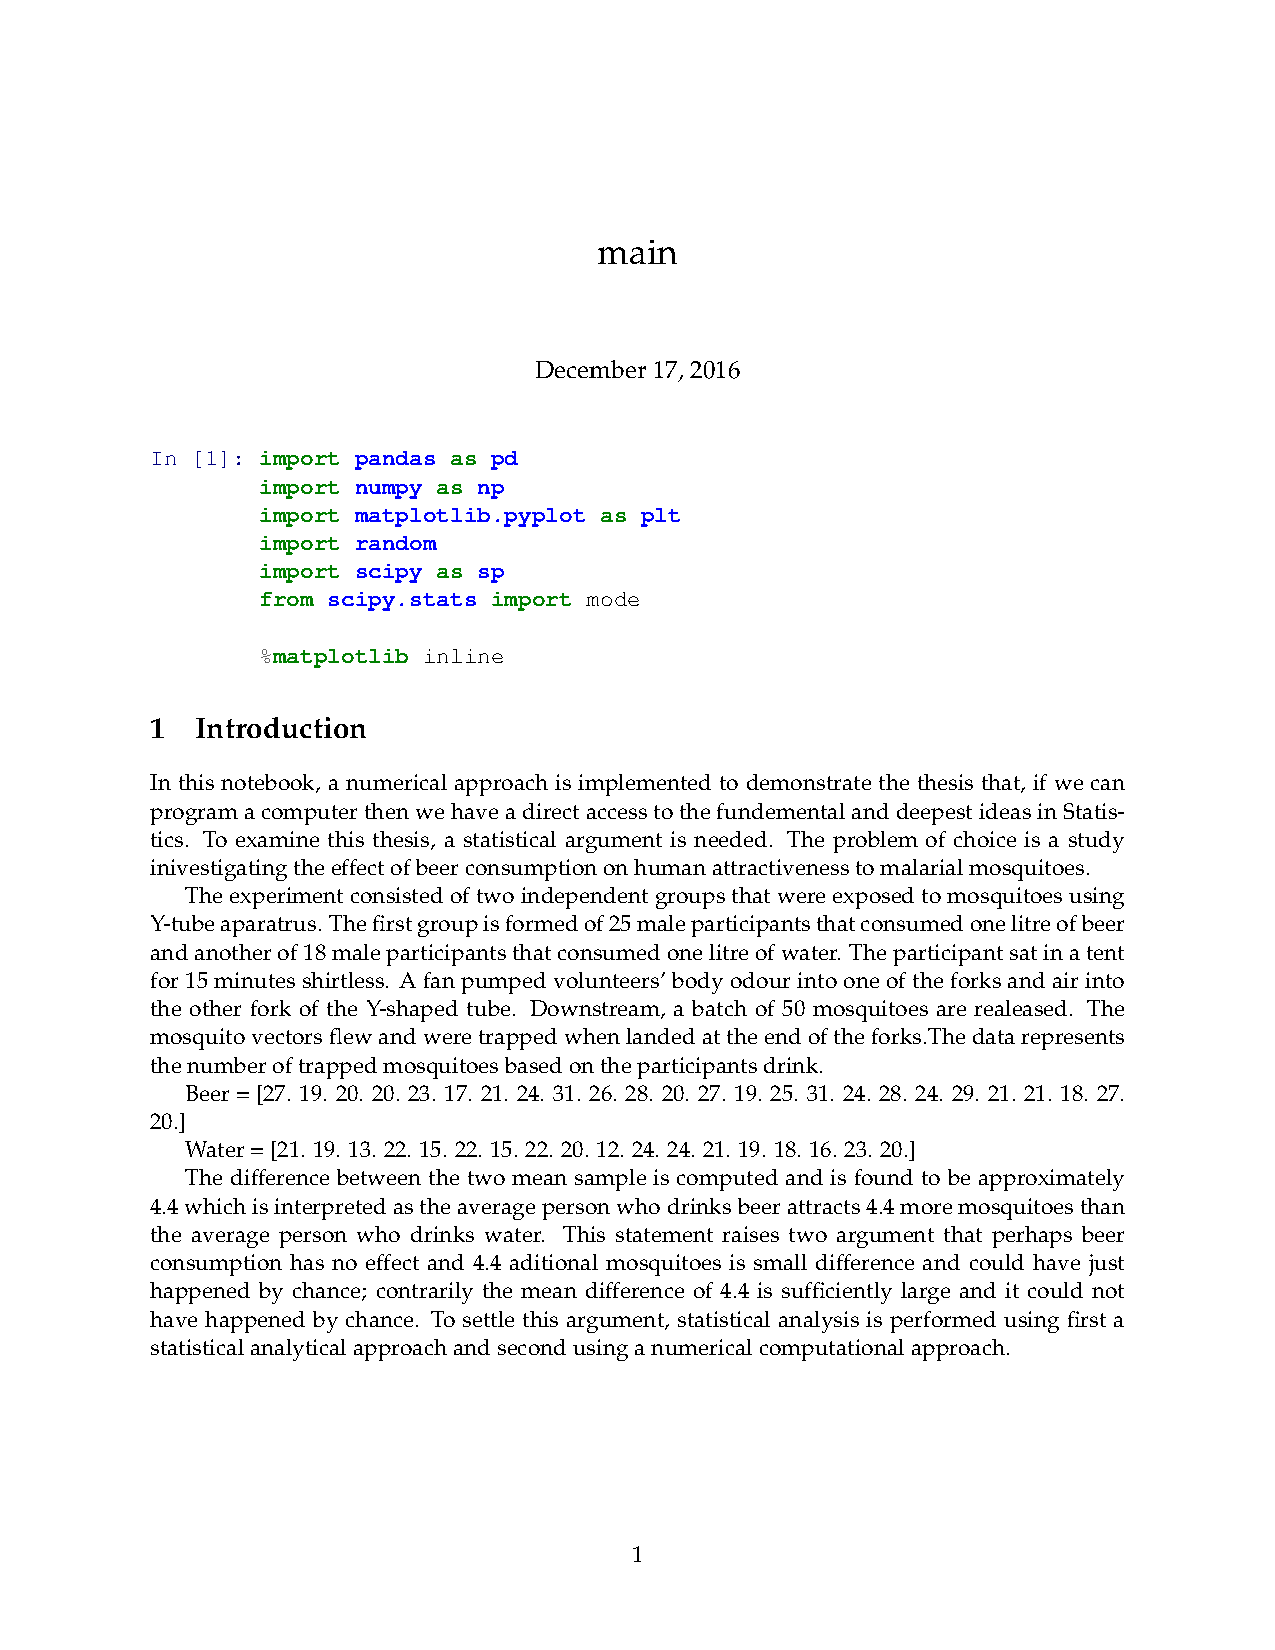
\includepdf[pages=-]{main.pdf}


\cleardoublepage
\bibliographystyle{plain}
\addcontentsline{toc}{chapter} {Bibliography}
\bibliography{./bibliography/sources}


\end{document}




